\title{\textbf{Christian perspectives on sustainability: \\
		The need for numerical answers to philosophical questions.}}
% Sustainability challenges and managing tradeoffs: engineers' need for numerical answers to philosophical questions 
\author{
		% Authors must be italicized.
        % \emph{Jeremy Van Antwerp} and \emph{Matthew Kuperus Heun}%
% \footnote{
% Engineering Department,
% Calvin College,
% Grand Rapids, MI, 49546, USA}
}

\documentclass[12pt]{article}

% CEC papers should be set in Times New Roman.
% https://tex.stackexchange.com/questions/153168/how-to-set-document-font-to-times-new-roman-by-command
% suggests the following.
\usepackage{mathptmx}             % For Times New Roman font (or a close approximation thereof).
\usepackage[margin=1in]{geometry} % For 1-inch margins all around.
\usepackage[document]{ragged2e}   % For left justification.
\usepackage{parskip}              % For double-spacing between paragraphs.
\usepackage{nopageno}             % To eliminate page numbers.
% For MLA bibliography. See https://www.ctan.org/pkg/biblatex-mla?lang=en for details.
\usepackage[american]{babel}
\usepackage{csquotes}
\usepackage[style=mla-new]{biblatex}
\addbibresource{JVAMKH.bib}
\usepackage[inline]{enumitem}  % For inline enumerate* lists

\usepackage{titlesec}             % To change formats of section titles, etc.
\titleformat*{\section}{\normalsize}
\titleformat*{\subsection}{\normalsize}
\titleformat*{\subsubsection}{\normalsize}
\titleformat*{\paragraph}{\itshape} % Set paragraph titles to italics
\usepackage{abstract}             % Set characteristics of the abstract
\setlength{\absleftindent}{0in}   % Do not indent left side
\setlength{\absrightindent}{0in}  % Do not indent right side
\usepackage{url}
\setlength{\parindent}{0in}       % Do not indent the 1st line of paragraphs.
\setlength{\parskip}{12pt}        % Instead, add space between paragraphs.
\renewcommand{\abstractnamefont}{\normalfont\normalsize} % Unbold and regular size
\renewcommand{\abstracttextfont}{\normalfont\normalsize} % Unbold and regular size
\date{}                           % To eliminate the date in the title

% To include graphics
\usepackage{graphicx}

% Commands for editing.

\usepackage{xcolor}            % For colored text
\usepackage[normalem]{ulem}    % For \sout command (strikethrough)

% From https://tex.stackexchange.com/questions/130623/crossing-out-using-different-colour,
% Change the \sout color to red
\newcommand{\redsout}{\bgroup\markoverwith{\textcolor{red}{\rule[0.5ex]{2pt}{0.4pt}}}\ULon}

% Use these versions to display changes.
\newcommand{\del}[1]{\textcolor{gray}{\redsout{#1}}}
\newcommand{\ins}[1]{\textcolor{red}{#1}}
\newcommand{\rev}[2]{\del{#1}\ins{#2}}

% Use these versions for a clean copy.
% \newcommand{\del}[1]{}
% \newcommand{\ins}[1]{#1}
% \newcommand{\rev}[2]{#2}



\begin{document}
	
\maketitle

\begin{abstract}
\noindent
\ins{rewrite abstract from scratch. Later.}

\end{abstract}


%%%%%%%%%%%%%%%%%%%%%%%%%%%%%%%%%%%%%%%%%%%%%%%%%%%%%%%%%%%%%%
\section{Introduction}
\label{sec:introduction}
%%%%%%%%%%%%%%%%%%%%%%%%%%%%%%%%%%%%%%%%%%%%%%%%%%%%%%%%%%%%%%

Because of circumstances in our world today, 
concerns about environmental, economic, and social 
issues are significant. 
The concept of ``sustainability'' encompasses all three areas
with a view toward the future. 
(See Figure~\ref{fig:3_sustain}.)
One definition of sustainability is
``Sustainability emerges from choices that, on balance, 
promote economic vitality, social equity, and a flourishing natural environment 
both now and for generations to come''~\autocite{Calvin-College-2017}.
Sustainability is considered to be a ``grand challenge,'' 
and becoming more sustainable requires solving 
complex, multidisciplinary, and multifaceted problems
with both technical and non-technical, even philosophical, aspects. 
Sustainability challenges occur at both the 
macro level (where international coordination is needed for effective action) and
the micro level (where individual and person-to-person interactions can be beneficial). 

\begin{figure}
\centering
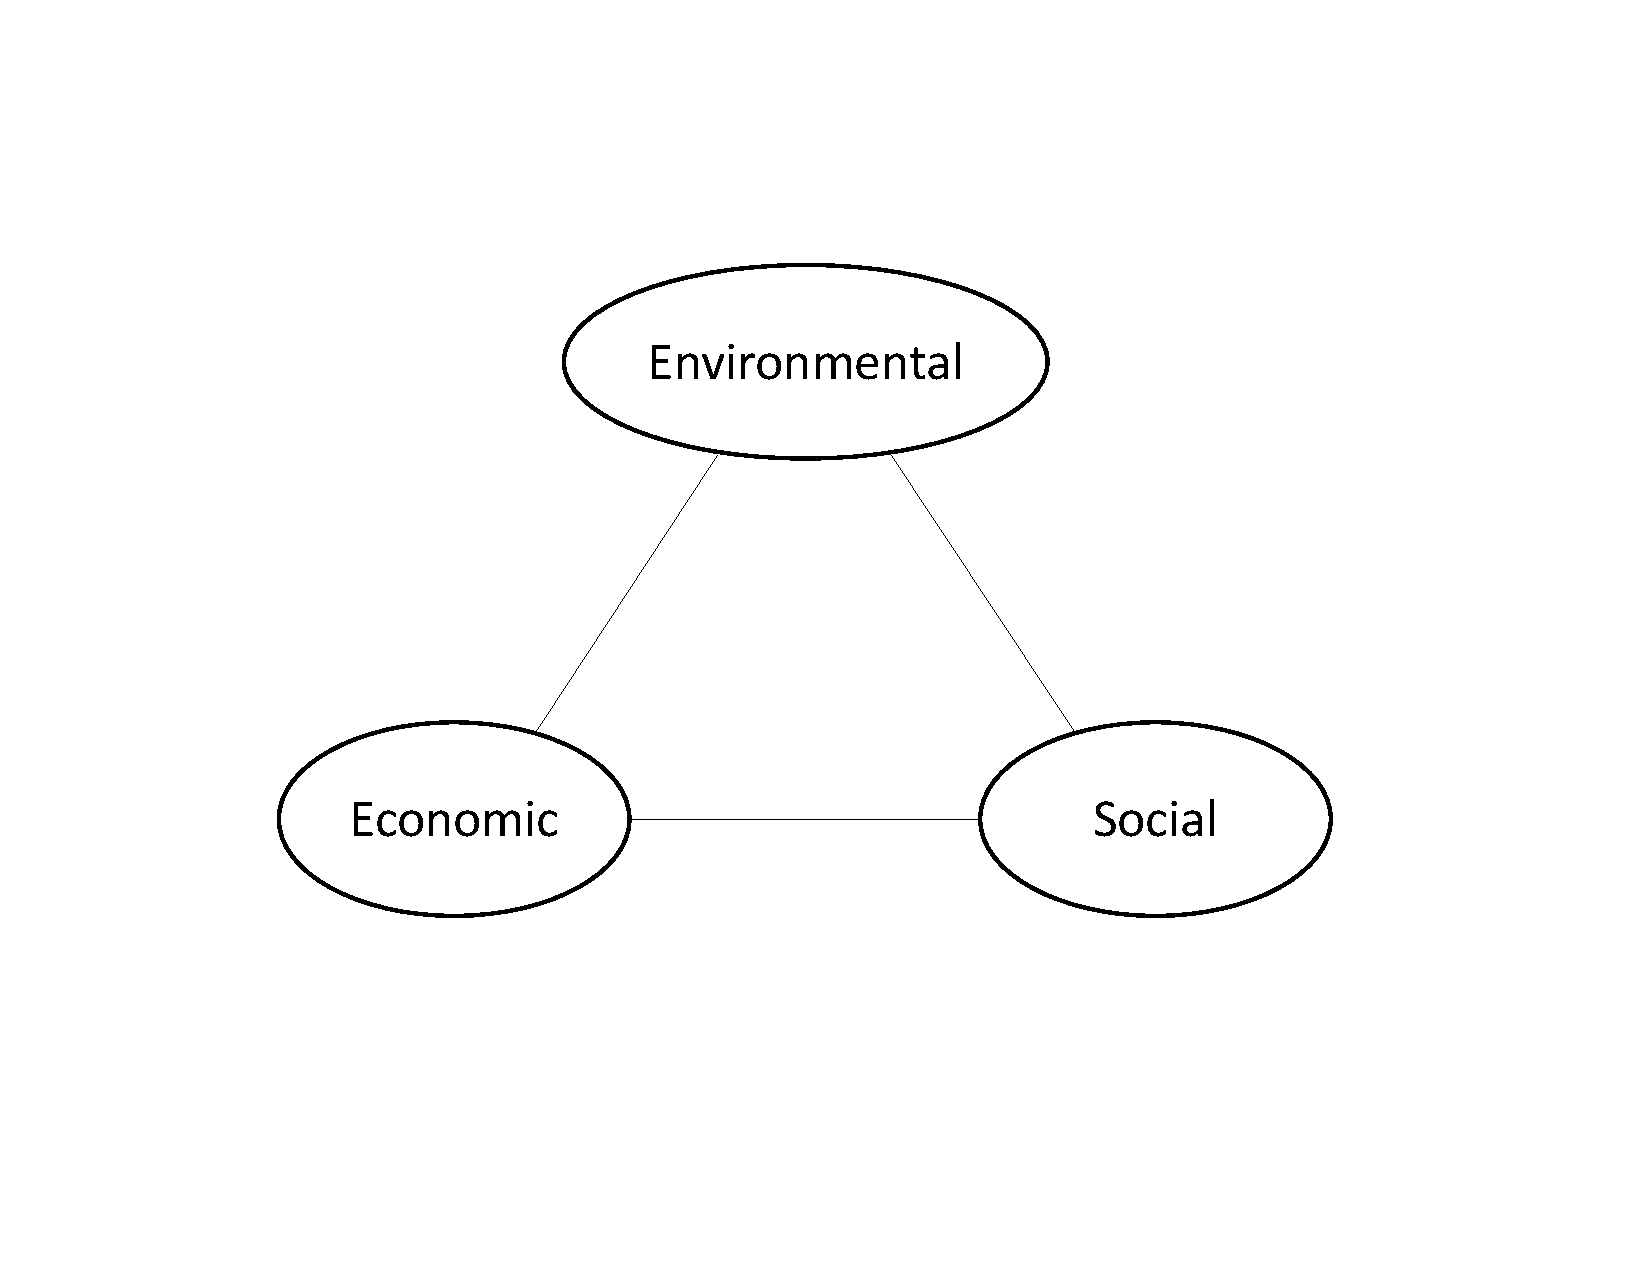
\includegraphics[width=0.75\linewidth]{figure_other/TriangleDiagram.pdf}
\caption{Three aspects of sustainability.}
\label{fig:3_sustain}
\end{figure}

In that milieu, 
we engineers design and operate the machines and systems that
%
\begin{enumerate*}[label={(\alph*)}]

  \item enhance the natural environment,

  \item generate economic growth by providing employment and economic output, and

  \item enhance society bring people together through communication technologies.

\end{enumerate*}
%
But we also design machines and systems that
%
\begin{enumerate*}[label={(\alph*)}]

  \item consume non-renewable materials and
        emit pollution, thereby contributing to environmental degradation,

  \item replace human workers, and

  \item foster online hate.        

\end{enumerate*}
%
Which direction a particular machine or system propels society is a function, in part,
of both its design and of the macro socio-economic policies that inform the design.
Because design is a central function of engineering, 
engineers have an important role to play in determining 
the sustainability of our future. 

But what guides engineers to make design choices that lead to sustainability?
And what guides policy-makers to make socio-economic-environmental
policy choices from which sustainability can emerge?
This paper explores two traditional answers to those questions:
the academic disciplines and theology/ethics.
But we begin by introducing several questions relevant to sustainability
that illustrate the need for guiding principles for design and policy.
We conclude with the claim that, as presently constituted, 
neither the disciplines nor theology/ethics is capable of providing
guidance to engineers and policy-makers
for developing machines or policies that move society in a sustainable direction.


%%%%%%%%%%%%%%%%%%%%%%%%%%%%%%%%%%%%%%%%%%%%%%%%%%%%%%%%%%%%%%
\section{Sustainability questions}
\label{sec:sustainability_questions}
%%%%%%%%%%%%%%%%%%%%%%%%%%%%%%%%%%%%%%%%%%%%%%%%%%%%%%%%%%%%%%

We begin with several example questions that arise in the sustainability space.
Each question is preceded by a few introductory sentences that set the stage for the 
sustainability issue.
Our list of questions is not exhaustive, nor is it meant to cover the entire sustainability triangle of 
Figure~\ref{fig:3_sustain}.
Rather, the questions illustrate the 
technical and non-technical, even philosophical, dimensions of sustainability challenges
and their
complex, multidisciplinary, and multifaceted 
nature. 
The questions are organized by their location in Figure~\ref{fig:3_sustain}
and are focused around the Social vertex.


%++++++++++++++++++++++++++++++
\subsection{Social}
\label{sec:social}
%++++++++++++++++++++++++++++++

Many sustainability questions exist at the social vertex of the sustainability triangle.
We start with a set of questions about population
and postulate that
for any given level of technological development, 
there must exist some upper limit to the human population level that the Earth can support. 
Calculating this upper limit is a technical problem with a 
(perhaps difficult-to-achieve)
but technical answer.  
But many non-technical questions flow from the postulate above.
%
\begin{enumerate}

  \item What is the ideal total population (which is less than or equal to maximum possible population)? 

  \item How should we manage for and arrive at this ideal population?
  
  \item Where should people live and what is the ideal geographical distribution of population?

\end{enumerate}
%
Answers to these questions expose human \emph{values}, which
inform relative preferences for 
social justice, 
standards of living, 
environmental versus economic and social tradeoffs, and 
the relative importance of the means versus the end.

But the questions about population issues 
at the social vertex do not end with the list above.
In fact, if decisions about numbers and locations of people are to be made,
rights emerge as a central issue.
What ``right'' do people have to food, water, air, medicine or health care, property, or a ``living'' wage? 
Where do these rights come from? 
What rights does the nonhuman world have, and what is the origin of nonhuman rights?
What rights do future generations have, and what is their origin?
What tradeoffs exist among these rights?
How do/should Christian assessments of tradeoffs change when costs and benefits
of decisions about population accrue to different (groups of) people?
Should decisions about population depend on whether many benefit at the expense of a few or
whether few benefit at the expense of many? 
Should decisions depend on whether benefits and costs accrue to different generations? 
Should decisions depend on the size of the benefit/cost matter? 
Does the number of people in the group matter? 
If so, what is a ``large enough'' difference to matter?

Additional questions at the social vertex go beyond population
to climate change and world energy supply, 
about which one hears many gloomy predictions.
In response, some say ``don't worry, it will all work out,'' while
others respond ``no it won't.'' 
To which ``prophets'' should we give credence?  
The Old Testament criteria for determining the legitimacy of prophets might provide guidance.
But as we learn from the Israelites, even when true prophets are discerned,
it can be very difficult to follow those prophets' advice. 

Finally, beyond prophets, the opinions of ordinary members of society (not prophets) 
should to be considered for designs and policies. 
But among non-prophets, we have topic experts and non-expert ``people in the street.''
Should the opinion of an expert researcher or technologist count for more 
than a non-expert ``man on the street'' on sustainability issues?
How about a government leader? 
Does it matter if the question under consideration is technical or nontechnical?


%++++++++++++++++++++++++++++++
\subsection{Social economics}
\label{sec:social_economics}
%++++++++++++++++++++++++++++++

Sustainability questions exist both at the vertices of Figure~\ref{fig:3_sustain}
(as illustrated by the Social vertex above) 
and along its edges.
To illustrate, we raise several questions along the edge between Economics and Social.

The questions emerge from a hypothetical policy proposal to ban all air travel.
Air travel is a particularly \emph{carbon intensive} activity on a per-person, per-mile basis. 
In 2013, air travel was responsible for about 3\% of US greenhouse gas emissions. 
% citation needed. EPA data appears to be offline now.
% see https://www.c2es.org/content/reducing-carbon-dioxide-emissions-from-aircraft/
% which cites Inventory of U.S. Greenhouse Gas Emissions and Sinks: 1990–2015 (U.S. Environmental Protection Agency, 2017)
Therefore, banning air travel could be an important step to making the world a more sustainable place. 

Engineers are well equipped to analyze some of the effects of this hypothetical policy. 
For instance, engineers could estimate additional carbon emissions 
from increases in use of other forms of transportation resulting from 
a ban on air travel. 
But there are other effects, too, many of which engineers are not well-placed to evaluate.
For example, 
GDP may decrease, because movement of goods from 
manufacturers to buyers will become more difficult.
There will be reduced air and noise pollution near airports, 
enhancing the aesthetics of nearby properties
and possibly increasing their economic value. 

Any policy change, such as banning air travel, 
will have \emph{direct} dollar-measurable impacts (such as change in GDP), 
\emph{indirect} but still dollar-measurable consequences (such as increased property values), and
consequences that \emph{aren't} measurable in dollars 
(such as improved aesthetics). 

The field of economic cost-benefit analysis attempts to express non-dollar-quantifiable 
social and environmental effects in dollar terms, 
thereby providing a consistent numeraire and allowing direct comparisons 
among social and economic (and environmental) effects. 

Questions arise here, especially for Christian engineers:
how should we evaluate design choices and policy prescriptions
whose effects are both dollar-quantifiable and non-dollar-quantifiable?

Furthermore, banning air travel might be considered a ``clean'' or ``ideal'' policy option. 
Other policy options could be classified as pragmatic, 
such as improving air travel energy efficiency. 
How should Christians navigate the space between ideal and pragmatic policy proposals
when both dollar-quantifiable and non-dollar-quantifiable effects are present?

Finally, some consequences of a ban on air travel 
could include the destruction of the air travel and 
reductions in ancillary industries (hotel, rental car, etc.).
The social effects of job losses would be sizable and 
would likely prompt implementation of remediation policies.
But would we do the same if job losses resulted from technological innovation or market forces?
Is not, why not?


%++++++++++++++++++++++++++++++
\subsection{Environmental social justice}
\label{sec:environmental_social_justice}
%++++++++++++++++++++++++++++++

Moving from the Social vertex to the Environmental vertex 
yields several questions related to social and environmental justice. 

Both the Old and New Testaments teach that Christians should care for those who are less fortunate,
(often by working to eliminate poverty). 
But we are also called to care for the nonhuman creation.
So how should Christians balance these two imperatives?
And how do we respond to the observation that alleviating poverty 
increases economic consumption, which has negative environmental consequences?

To make this tradeoff concrete, consider two examples.
First, suppose an impoverished farmer lives on the edge of a rainforest. 
Is it permissible for the farmer slash and burn the vegetation to create another subsistence farm?
Or put another way, would it be unjust to deny the farmer the opportunity to raise their family
out of poverty by reducing the size of the rainforest, 
thereby reducing the CO$_2$ absorbing capability of the planet?

Second, some say that coal mining is good,
because the benefits of employment provided by mining outweighs
any (potential) environmental harm caused by burning mined coal. 
How large does the social benefit need to be relative to the environmental cost 
for this to be true?
And, yet again, how are the non-dollar-quantifiable 
social and environmental costs and benefits to be weighed? 


%++++++++++++++++++++++++++++++
\subsection{Multifaceted}
\label{sec:multifaceted}
%++++++++++++++++++++++++++++++

The questions above clearly demonstrate that sustainability questions are multi-faceted.
And the sustainability triangle of Figure~\ref{fig:3_sustain} provides a useful means to organize those questions.

The multifaceted aspects of sustainability can be summarized in the following short questions:
%
\begin{itemize}

  \item How should the environmental, economic, and social aspects of sustainability be weighted against each other?
  
  \item What is the balance between the needs to the present and the needs of the future?	

\end{itemize}
%
As a society, we have \emph{de facto} arrived at answers to the summary questions above. 
However, there is increasing evidence to believe that our
answers will not lead to a sustainable future.
Given that our \emph{de facto} answers are not satisfactory, 
it may be prudent to re-examine how we have arrived at this place.
The values that guide our answers come from somewhere, and 
it is worthwhile to re-examine those sources.

We suggest that the values that guide the designs and policies that contribute to (or not) sustainability
are shaped by both academic disciplines and the combination of theology and ethics. 
In the two sections that follow, we examine each, 
starting with academic disciplines.


%%%%%%%%%%%%%%%%%%%%%%%%%%%%%%%%%%%%%%%%%%%%%%%%%%%%%%%%%%%%%%
\section{Sustainability and the academic disciplines}
\label{sec:sustainability_and_the_academic_disciplines}
%%%%%%%%%%%%%%%%%%%%%%%%%%%%%%%%%%%%%%%%%%%%%%%%%%%%%%%%%%%%%%

As the questions above illustrate, 
moving toward sustainability is challenging, 
because environmental, economic, and social challenges  
are complex, multidisciplinary, and multifaceted, with 
technical and non-technical, even philosophical, aspects.
But what guides engineers to make design choices that lead to sustainability?
And what guides policy-makers to make socio-economic-environmental
policy choices from which sustainability can emerge?

A traditional answer in the secular world is ``the academic disciplines,'' 
which are both generators of and repositories for accumulated human knowledge
about a problem domain.
Of course, there are academic disciplines 
at each vertex of the sustainability triangle (Figure~\ref{fig:3_sustain}):
Environmental Studies (or Ecology, Biology, etc.) for the Environmental vertex, 
Economics for the Economic vertex, and 
Sociology for the Social vertex.
But, as shown above, difficult sustainability-related 
challenges exist across disciplinary boundaries and, by definition,
cannot be addressed or solved by a single vertex discipline alone.

In a hopeful interdisciplinary sign, 
disciplines have emerged along the edges of Figure~\ref{fig:3_sustain}.
(See Figure~\ref{fig:3_sustain_with_edge_disciplines}.)
Environmental Economics was founded in the 1960s,
focusing on valuation of ecosystem services and 
internalization of externalities associated with environmental degradation.
In the 1970s, Environmental Sociology emerged along the Environmental--Social edge 
to study interactions between society and the natural environment. 
Along the Social--Economic edge, Socioeconomics (also called Social Economics) 
emerged in the early 1980s
to study interactions between societies and their economies.
Ecological Economics, founded in the late 1980s, 
is a reaction to the perceived narrowness of environmental economics, 
emphasizing that the economy as a subsystem of the environment.
Fittingly, there are journals for each edge:
the \emph{Journal of Environmental Economics and Management}, 
\emph{Environmental Sociology}, 
the \emph{International Journal of Social Economics} and the \emph{Journal of Socio-Economics}, and
\emph{Ecological Economics}.

\begin{figure}
\centering
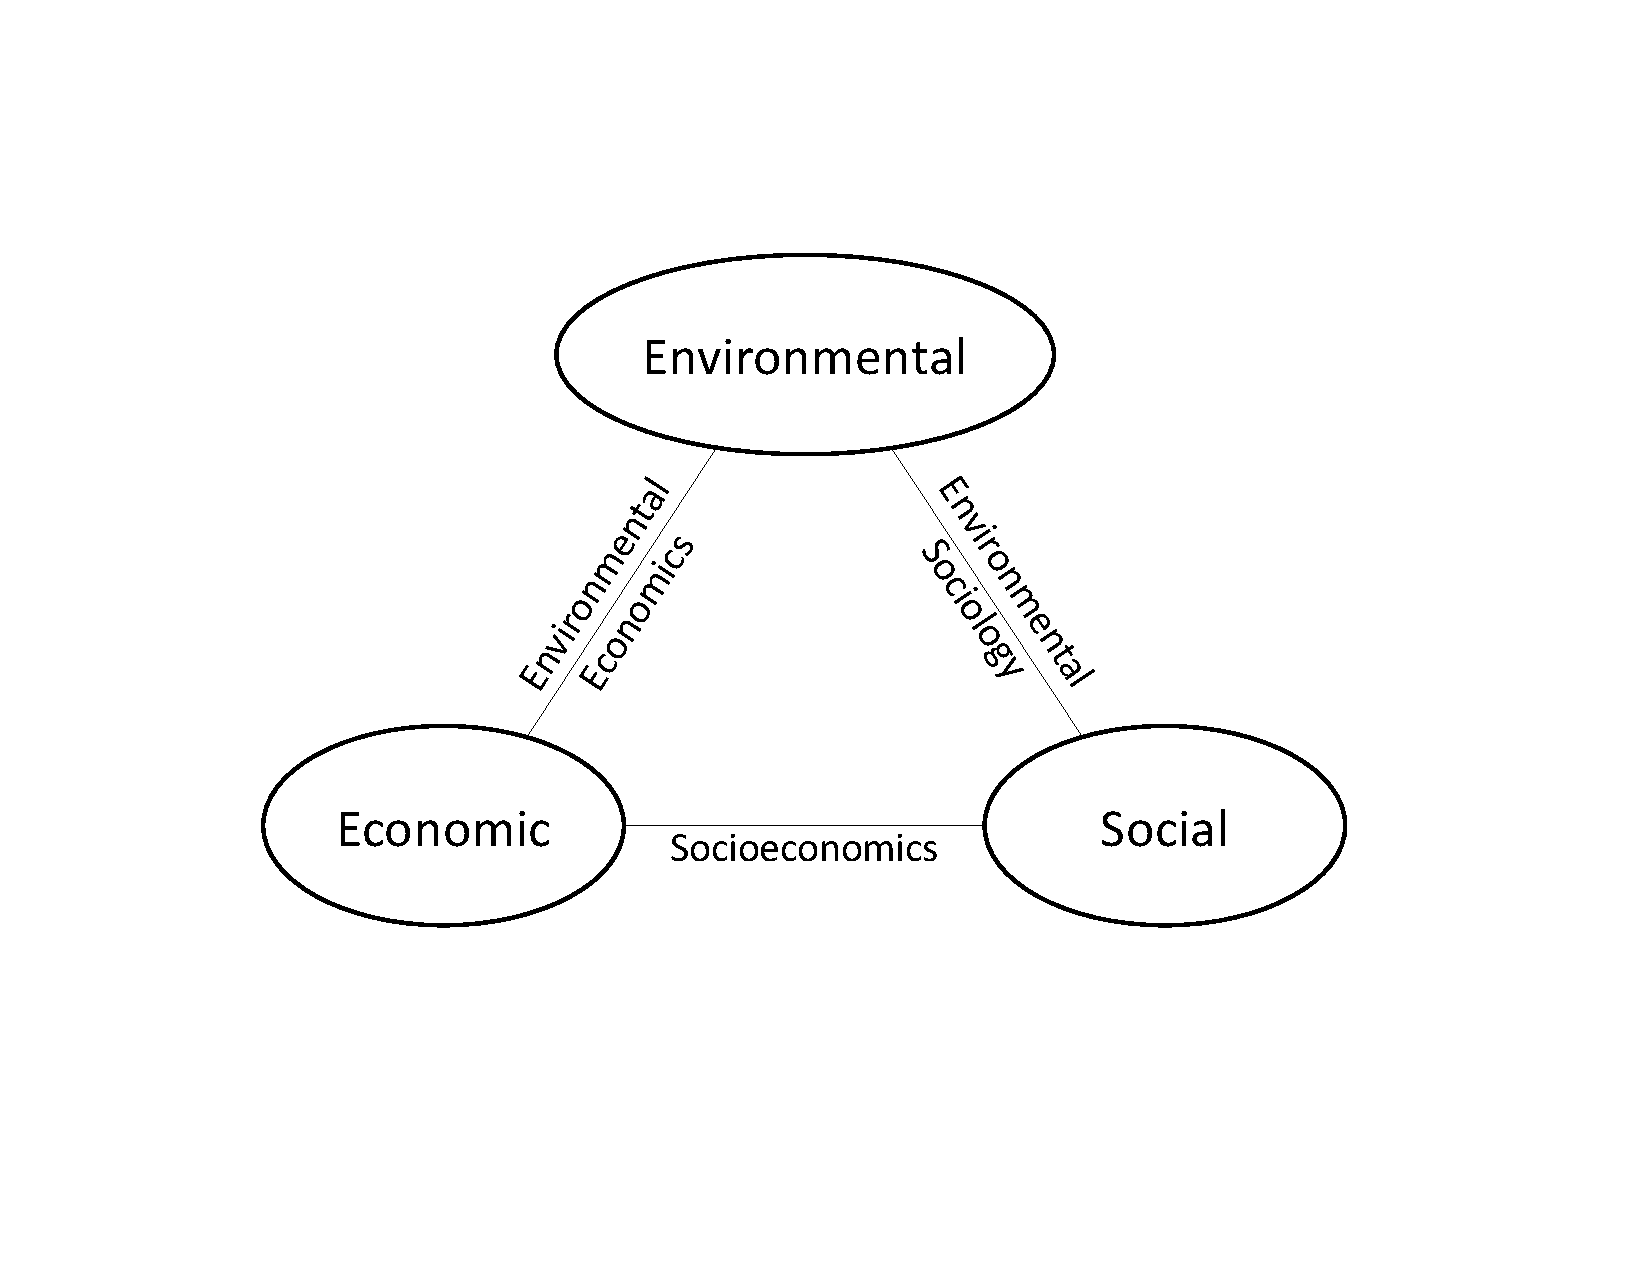
\includegraphics[width=0.75\linewidth]{figure_other/TriangleDiagramWithDisciplines.pdf}
\caption{Three aspects of sustainability with edge disciplines.}
\label{fig:3_sustain_with_edge_disciplines}
\end{figure}

However, our assessment of the vertex and edge disciplines,
as presently constituted,
is that they are not up to the challenge of answering the hard questions on sustainability,
some of which are provided in Section~\ref{sec:sustainability_questions}.

The edge disciplines often assume that difficult tradeoffs can be routed around (or don't exist), 
i.e., they assume that sustainability isn't a zero-sum game. 
For example, 
much of the literature on sustainability 
assumes that it is possible to have both ``development,'' 
by which it is meant lifting people out of poverty,
and environmental conservation. 
For example, ``Humanity has the ability to make development sustainable ... widespread poverty is no
longer inevitable if policies that nurture and favor growth are adopted and implemented'' \cite{Ngome2015}.

Sometimes the edge disciplines are right, particularly at the micro level.
For example, technical innovation sometimes can both 
improve living standards and reduce energy consumption
(e.g., by insulating old homes).
But sometimes, and particularly at the macro level,
sustainability really is a zero-sum game, and 
prosperity and conservation are really at odds.
For example, you can't \emph{both} use fossil fuels and conserve fossil fuels.
Economic activity requires input of resources
and produces outputs such as pollution. 
And fundamentally, economic growth is itself unsustainable; 
at some level of economic activity,
the Earth will not be able to supply the inputs needed and/or 
absorb the wastes our economies produce.
Too often the edge disciplines fail to grapple with this larger picture.

Another common error in the sustainability literature of the edge disciplines
is the assumption that it will be possible to move 
from our current situation to a sustainable future. 
These studies look forward without
serious consideration of whether a sustainable future state 
is practically, physically, and/or technically achievable. 
One helpful question to discern fanciful or wishful thinking
is ``what would have to be true for this to happen?''
For example, it is generally understood that a carbon-neutral 
energy sector is necessary for sustainability.
What would have to be true for the world to transition to an energy sector 
that doesn't emit greenhouse gases?
%
\begin{itemize}

  \item There would have to be massive investments in renewable-energy generation. 
        Replacing all coal-fired power plants in the United States (1.2 trillion kW-hrs/yr) %citations needed.
        with solar generation would require about 4 million acres of land 
        (about 0.2\% of the US land area, or about half the state of Maryland) 
        and an investment of \$2 trillion, which is about one tenth of the annual US GDP. 

  \item There would have to be massive energy storage. 
        Eighteen to 40 hours worth of electricity storage would 
        have been needed for a fully renewable grid to get the Midwest and Northeast 
		through the January 27--February 2, 2019 polar vortex \cite{wood2019}.
		
  \item There would have to be massive changes to the electricity distribution grid.
  
  \item There would be massive disruptions to large sectors of the economy. 
        Oil and gas exploration and extraction would be almost entirely diminished.
		Gas stations would be out of business -- or maybe changed to charging stations.

\end{itemize}

Furthermore, these edge disciplines exist, almost by definition, 
on the fringes of the vertex disciplines:
E.g., Ecological Economics is not considered ``real'' economics by many economists.
Even if the edge disciplines had the right answers to sustainability questions, 
they would not affect the vertex disciplines. 

Thus, we do not see how the academic disciplines, as presently constituted,
will provide answers to important sustainability questions.
Their vision is not broad enough to be policy-releavant at the macro scale, 
they too-rarely grapple with the non-zero sum aspects of sustainability, and
they too-often fail to explore the practical, physical, and/or technical
constraints on sustainability policies. 


%%%%%%%%%%%%%%%%%%%%%%%%%%%%%%%%%%%%%%%%%%%%%%%%%%%%%%%%%%%%%%
\section{Sustainability and worldviews}
\label{sec:worldviews}
%%%%%%%%%%%%%%%%%%%%%%%%%%%%%%%%%%%%%%%%%%%%%%%%%%%%%%%%%%%%%%

If old and new academic disciplines are not up to the task 
of providing guidance to engineers and policy-makers
on sustainability challenges, 
perhaps theology and ethics and the worldviews inspired by them
will be beneficial.
Our starting point for this exploration is the thesis that 
all things (even the academic disciplines discussed 
in Section~\ref{sec:sustainability_and_the_academic_disciplines})
are informed by worldviews.
Worldviews, in turn, are both shaped by and contribute to religions, theologies, and ethics.
Sustainbiltiy challenges, too, exist within, are surrounded by, and are informed by 
all of the above:
worldviews, religions, theologies, and ethics.
To illustrate the point, we surround the sustainability triangle and edge disciplines with the 
milieu of worldviews, religions, theologies, and ethics in Figure~\ref{fig:3_sustain_with_worldviews}.
In this section, we'll use the shorthand ``worldviews'' to mean the milieu 
as shown in Figure~\ref{fig:3_sustain_with_worldviews}.
Our focus below is on Christian worldviews 
associated with the vertices of the sustainability triangle, 
first discussing ``Environmental'' and ending with 
``Economic'' and ``Social'' together.

\begin{figure}
\centering
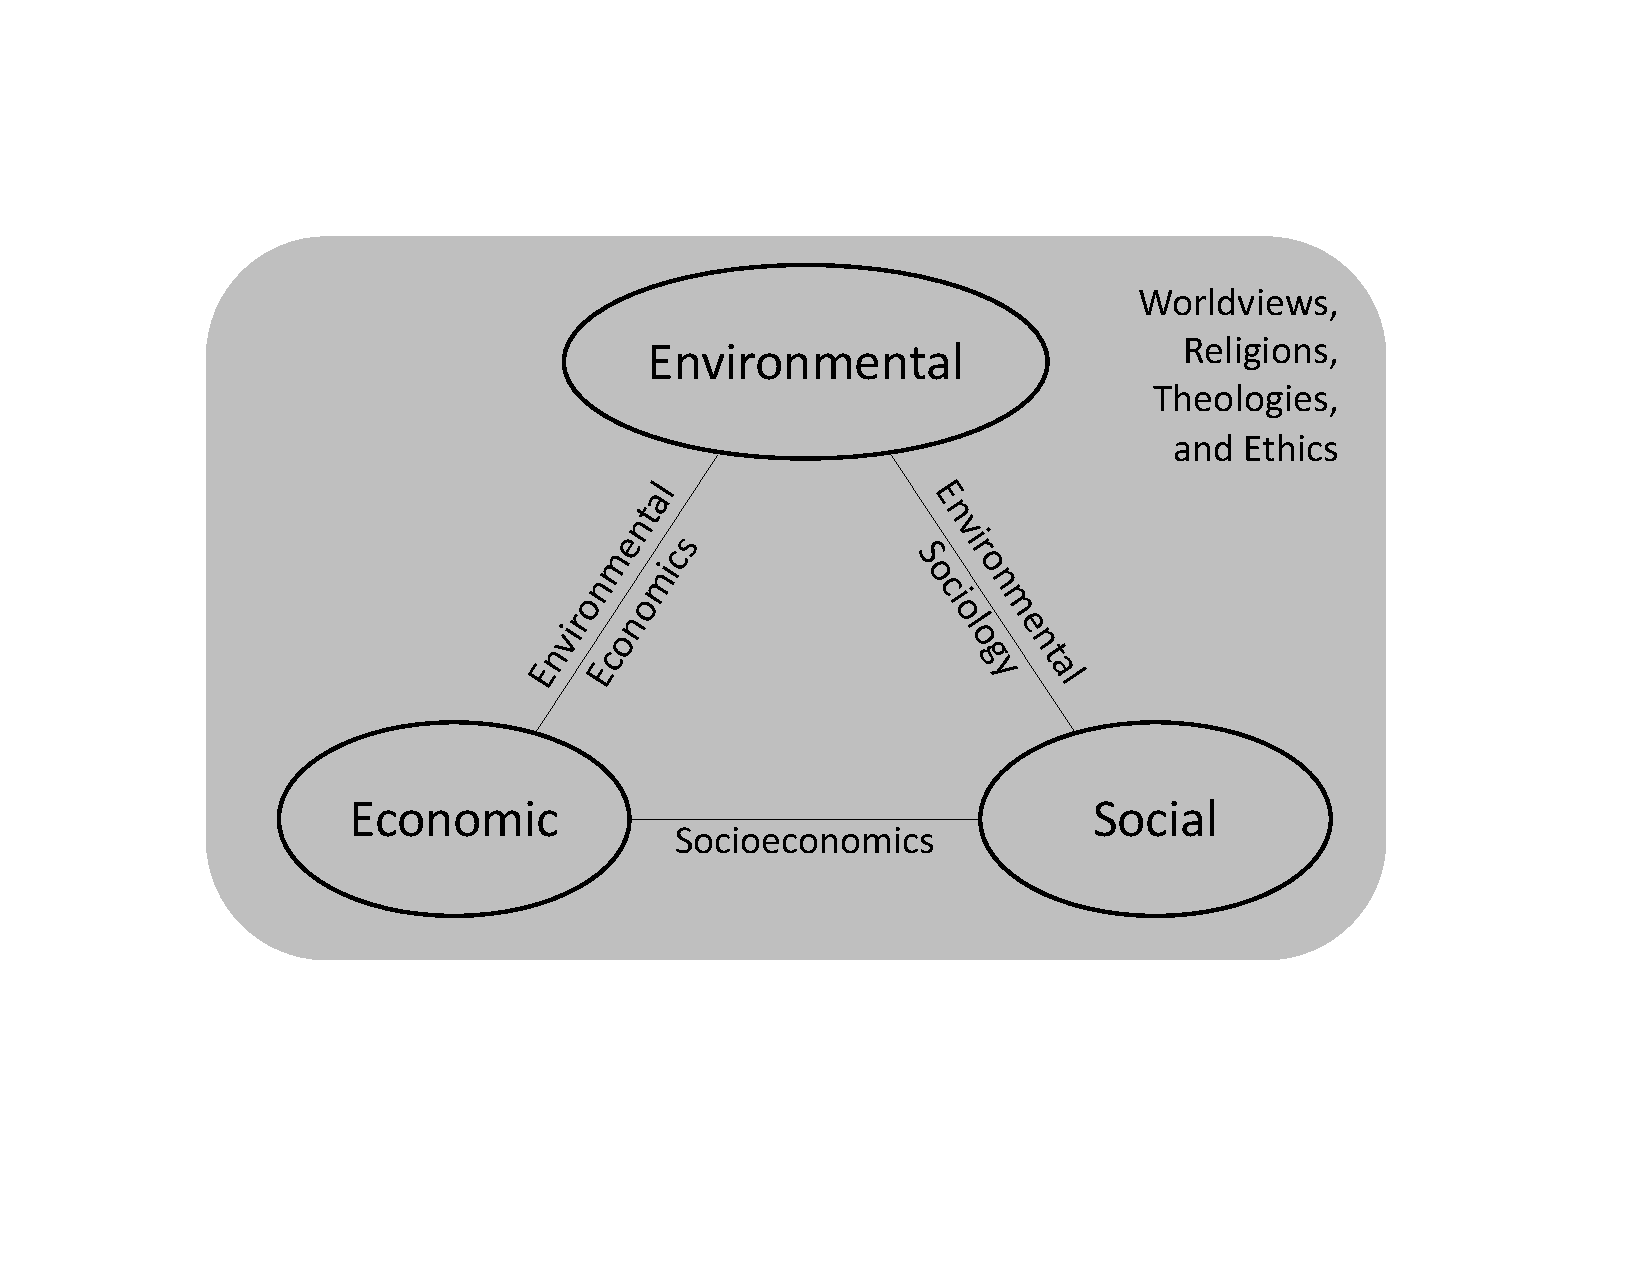
\includegraphics[width=0.75\linewidth]{figure_other/TriangleDiagramWithTheology.pdf}
\caption{Three aspects of sustainability surrounded by worldviews, religion, and theology.}
\label{fig:3_sustain_with_worldviews}
\end{figure}


****** Matt ended here ****************


%++++++++++++++++++++++++++++++
\subsection{Environmental worldviews}
\label{sec:environmental}
%++++++++++++++++++++++++++++++

The book \emph{Ecologies of Grace} \autocite{Jenkins:2008}
provides a topology of Christian thought regarding the 
nonhuman creation and the
environmental aspect of sustainability.
In it, Willis Jenkins identifies three schools of thought:
stewardship, 
eco-justice, and 
ecological spirituality,
which loosely correspond to 
Reformed (or evangelical protestant), 
Roman Catholic, and 
Eastern Orthodox 
traditions.
To Jenkins' three, we add a fourth:
consumptive economic prosperity and
the conservative evangelical tradition. 
These four schools of thought 
span a wide range of Christian stances toward the nonhuman creation
and 
consequently outline a range of possibilities 
for Christian responses to environmental sustainability challenges.

%..............................
\paragraph{Stewardship} 
\label{sec:stewardship}
%..............................

The stewardship school of thought 
emphasizes that all of human existence
is a response to God's redemptive acts
and God's providence to humans.
Knowing God leads to vocational responsibility 
to care for nonhuman creation,
the means by which God provides for humankind 
% For some reason, we need to include this citation twice to get both author and page number to appear.
(\textcite{Jenkins:2008} \textcite[19]{Jenkins:2008}). 
Thus, all human work to care for the creation 
is seen as service to the Creator
out of gratitude for redemption (\textcite{Jenkins:2008} \textcite[77]{Jenkins:2008}).
\emph{Earthkeeping} \autocite{Wilkenson:1980aa} provides a cogent summary
of the importance of stewardship for Reformed Christians doing creation care.

The idea of stewardship is a reaction 
against themes of human dominion over the nonhuman creation
(often implemented as \emph{domination})
that emerge from some interpretations of the creation stories in Genesis.
Christians in the stewardship tradition are inspired by an interpretation of Gen~1:26–28 in which 
``the proper exercise of dominion yields shalom: the flourishing of all creation'' \autocite{BoumaPrediger:2019}.
As such, the first order of business for stewardship-minded Christians
is to act as shalom-building caretakers of God's creation.

The \emph{stewardship} viewpoint acknowledges that tradeoffs
are present in every policy and in every decision. 
So, in an engineering sense, 
Christian environmental stewardship could be considered an optimization problem
in which policies that bring about the most good 
are to be preferred.
Furthermore, designs and policies can be critiqued 
based on the \emph{process} by which they emerged.
Were all voices heard? Was the assessment of tradeoffs accurate?
Who decides what goods matter most is important, and 
all voices should be heard on each matter.
Ignoring or disregarding voices is dangerous,
since injustices could result.
Humans will be persuaded on the right course of action
for sustainability policies by weighing the tradeoffs 
among environmental, economic, and social factors.

Weakness of the stewardship approach are
%
\begin{itemize}

  \item deliberation needs to be exhaustive and can be exhausting,

  \item imperfect information can lead to disastrous results,
  
  \item biblical support for stewarding creation is limited,
  
  \item stewardship causes separations between God and the creation and between 
        humans and the nonhuman creation, and
		
  \item stewardship leads to an instrumental view of the nonhuman creation.

\end{itemize}

Some argue that we need to move beyond stewardship 
for effective Christian environmental thought and action~\autocite{WarnersHeun:2019aa}.


%..............................
\paragraph{Eco-justice} 
\label{sec:eco-justice}
%..............................

The eco-justice school of thought 
emphasizes that God's grace reveals the creation's 
inherent integrity \autocite[19]{Jenkins:2008}, 
giving it natural value and inherent moral standing~\autocite{Joldersma:2019}. 
Thus, Christians must respect creation's inherent value and 
respond to its moral standing in all activities.
If the nonhuman creation can't speak for itself, 
we must speak for it and defend it when necessary.

The \emph{Laudato Si} encyclical \autocite{Pope-Francis:2015aa} 
is a clear enunciation of Roman Catholic thought
on environmental sustainability issues.
In it, Pope Francis portrays the nonhuman creation as a
``sister with whom we share our life and a beautiful mother who opens her arms to embrace us''
(\textcite{Pope-Francis:2015aa} \textcite[3]{Pope-Francis:2015aa}).
However, our sister and mother
``cries out to us because of the harm we have inflicted on her 
by our irresponsible use and abuse of the goods with which God has endowed her''
(\textcite{Pope-Francis:2015aa} \textcite[3]{Pope-Francis:2015aa}).
With this framing, the Holy Father evokes centuries of Catholic social teaching
about the need to support the oppressed, the poor, and the vulnerable.
Christians in the eco-justice tradition would point to the beatitudes (Lk 6) 
for reminders of the inherent value of those who are oppressed.
The first order of business for eco-justice-minded Christians
is to bring justice to the nonhuman creation, to right the wrongs
of abuse that humans have heaped upon the nonhuman creation.

The eco-justice point of view
weighs the environmental justice of any design or policy
against the possible economic injustice of depriving others
(especially the poor). 
Eco-justice adherents would be more likely to approve a design or support a policy if it
were accompanied by a robust and reliable way to ensure that one people group or another
are not disproportionally affected.

Furthermore, eco-justice is based upon the moral standing of the nonhuman creation,
meaning that the nonhuman creation itself must be given a voice.
To properly evaluate sustainability tradeoffs,
someone must be empowered to speak for the nonhuman creation and
give voice to unjust and unfair aspects of policies and decisions
that have implications for sustainability and the nonhuman creation.
Humans will pursue the right course of action on sustainability issues
when someone speaks eloquently and forcefully for the
those who can't speak for themselves, including the nonhuman creation.

A significant weakness of the eco-justice point of view is that,
in practical terms, time and attention are limited.
``Speaking up'' for the nonhuman creation is a tall order for most humans.


%..............................
\paragraph{Ecological spiritualities} 
\label{sec:ecological_spiritualities}
%..............................

The ecological spiritualities school of thought 
highlights the union between all of creation and God.
Consequently, and by virtue of both owing their existence to the creator,
there is a radical connectedness among all human and nonhuman creatures 
in the creation~\autocite[93]{Jenkins:2008}.

The speech ``To Commit a Crime Against the Natural World Is a Sin'' 
\autocite[133-136]{Bartholomew-I-of-Constantinople:2011aa}
provides an excellent summary of the ecological spiritualities point of view
on the nonhuman creation.
In it, Bartholomew states,
``at the heart of the relationship between man and environment 
is the relationship between human beings.
As individuals, we live not only in vertical relationships to God 
and horizontal relationships to one another, but 
also in a complex web of relationships that extend throughout
our lives, our cultures, and the material world.''
(\textcite{Bartholomew-I-of-Constantinople:2011aa} 
\textcite[133--134]{Bartholomew-I-of-Constantinople:2011aa})
Thus, any harm done to the nonhuman creation is a harm done to other human beings, but
any good done to the environment is a good done to humans, 
and praiseworthy. 
In the ecological spiritualities school of thought, 
tradeoffs among the environmental, economic, and social realms of sustainability
fade into the background. 

The first order of business for Christians in the ``ecological spiritualities'' mindset 
is asceticism, self-restraint for the good of the nonhuman creation and for others.
Asceticism will lead to practices that look much like conservation of the nonhuman creation.

A weakness of the ecological spiritualities school of thought
is that by assuming away tradeoffs,
it fail to grapple substantively with tradeoffs
among the three aspects of sustainability
in real-world situations.


%..............................
\paragraph{Consumptive economic prosperity} 
\label{sec:consumptive_economic_prosperity}
%..............................

The consumptive economic prosperity school of thought 
holds that the nonhuman creation is resilient, robust, and self-correcting.
Furthermore, its well-being is assured by God, 
because part of the ``goodness'' that God designed into the creation
is robustness to human actions; 
God is always in control.
In this school of thought, human well-being is paramount. 
Thus, humans are to be consumers of the nonhuman creation 
to provide economic prosperity and
lift people out of poverty.
Documents from the Cornwall Alliance 
provide a summary of conservative evangelical thinking on creation care issues
\autocite{Cornwall:2006aa}.

People with the \emph{consumptive economic prosperity} worldview
will claim that any environmental degradation caused by humans will be fixable,
given sufficient economic resources with guidance provided by the free market's invisible hand.
Thus, reducing economic prosperity will, ultimately, be bad for the environment, because
we will have fewer economic resources with which to address environmental damage.
Thus, the first order of business in the consumptive economic prosperity school of thought
is economic growth. 

Weaknesses of this approach to the nonhuman creation include:
%
\begin{itemize}

  \item reluctance to grapple with human impacts on the nonhuman creation and 

  \item reduction of the nonhuman creation to economic terms.

\end{itemize}


%++++++++++++++++++++++++++++++
\subsection{Economic and Social Perspectives}
\label{sec:economic_and_social}
%++++++++++++++++++++++++++++++

Worldviews on economic and social issues are often grouped together, and
we follow that tradition here. 
An instructive axis on which to consider the economic and social aspects of sustainability
is the range between ``Individualistic'' and ``Collectivistic'' points of view, 
as shown in Figure~\ref{fig:table}.
Christians of all stripes (denomination, gender, ethnicity, nationality)
hold individualistic or collectivistic points of view, 
so we do not associate these perspectives with any particular branch of Christianity
or group of Christians.
(In fact, political persuasion is a more-accurate predictor of location along the 
individualistic---collectivistic axis than denomination or other factors.
**** Do we want to make this claim? ---MKH)
After discussing the range of Christian economic and social perspectives,
we illustrate our points by applying the perspectives to the 
tragedy of the commons. 

\begin{figure}
\centering
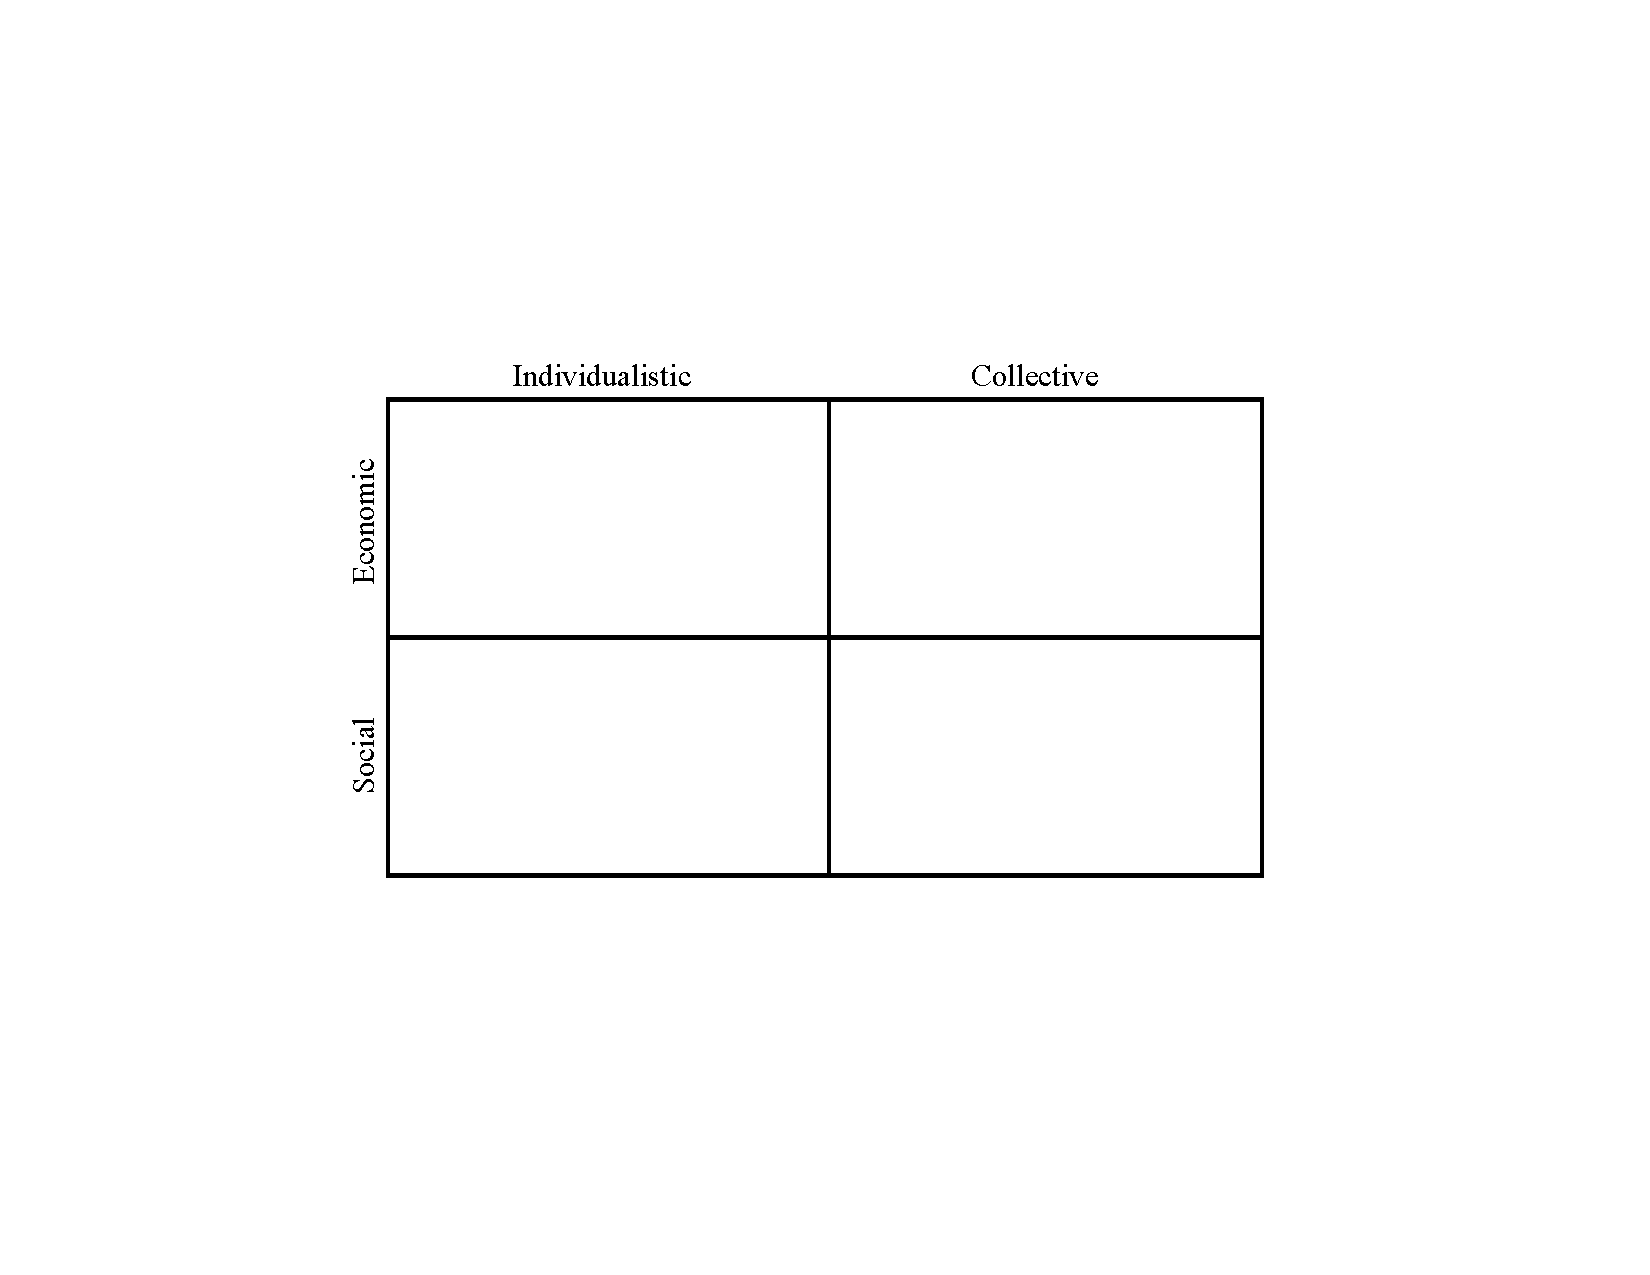
\includegraphics[width=0.75\linewidth]{figure_other/QuadTable}
\caption{Table for individualistic and collectivistic views on economic and social issues.}
\label{fig:table}
\end{figure}

Biblical teachings in the economic and social realms are often recognized 
as two sides of the same coin, 
for example in Micah 2:1-2, 
where the unjust deeds are economic in nature. 
Furthermore, Biblical teaching on economics and justice does not provide a
systematic, over-arching theory (macro),
but rather focuses on individual interactions (micro).
(One exception to this pattern is the Old Testament sabbatical/jubilee system 
of canceling debt and returning property.
In modern economic terms, canceling debts and returning property would serve to minimize 
\emph{income inequality} and ensure that there was universal access to the \emph{means of production}.
**** Insert Matt's really important comment here.
What was that comment again? ---MKH ****)
Indeed, much of the Bible's
teaching on money relates to generosity to the poor. 
Numerous Old and New Testament passages instruct God's faithful to
give generously to the poor, the disadvantaged, and the marginalized, 
where ``giving'' is meant to be some combination of 
money (traditionally called ``alms''), 
material goods (such as food or clothing), and 
justice or fairness.
We might say that the Bible majors on the micro,
while sustainability concerns are focused on the macro.

Some Christians view wealth itself as a root of evil. 
This view goes beyond merely \emph{love} money
being the root of evil (I Tim 6:10). 
Proponents of the view that money itself is a source of evil would point to Jesus
telling the rich young man to sell all his possessions and give to the poor and 
Jesus' further comment that it is easier
for a camel to go through the eye of a needle than 
for a rich man to enter the kingdom of God (Mt 19:16-30, Mk 10:17-31, Luke 18:18-30). 
At the other end of the spectrum of Christian thought, 
worldly wealth is seen as God's blessing, 
even an indication of God's favor.

In terms of modern economic views, Christians hold a wide range of positions. 
Some Christian traditions advocate a
collectivistic economic arrangement, in imitation of the early church (Acts 2:42-46). 
Examples range from monastic orders such as
might be found in Roman Catholic or Eastern Orthodox traditions 
to the Hutterite and Bruderhof communities, 
which come from an Anabaptist tradition. 
At the other end of the economic spectrum, many Christians advocate for an economic system
based on individual ownership and freedom of enterprise. 
Some key verses that support a more individual view include the comments 
``Didn’t it belong to you before it was sold? And after it was sold, 
wasn’t the money at your disposal?'' (Acts 5:4) and 
Paul's instruction that we should work to eat (2 Thes 3:10) and to share with those in need (Eph 4:28).
Thus, Christians hold a range of views from economic thought from individualistic to collectivistic.

Likewise, Christian social perspectives can stress individual freedom or collective behavior.
A liberal (individualistic) approach to providing for poor widows 
would be tied to instruction that widows should be 
provided for, first of all, from their own families (1 Tim 5:4). 
The collectivistic approach is represented by the group effort of caring for widows 
at the beginning of Acts 6.

To illustrate the individualistic and collectivistic approaches to the economic and social 
aspects of sustainability, 
we apply those perspectives to a classic sustainability problem, 
the tragedy of the commons. 
The term ``tragedy of the commons'' was popularized by Hardin \autocite{Hardin68} 
and provides a shorthand reference to situations where 
%
\begin{enumerate*}[label={(\alph*)}]

  \item there is equal and open access to a resource or pool of resources and

  \item it is in the rational self-interest of
		every individual to maximize their use of the resource, even if this results in the net effect of destroying the
		resource itself through over exploitation.

\end{enumerate*}
% 
This class of problems is recognized as ``having no technical solution.''
Instead, sustainable solutions emerge from decisions (policies) 
that address all vertices of the sustainability triangle:
environmental, economic, and social.

As originally stated, each herder has incentive 
to add more animals to his or her flocks grazing on the common land, because
the benefits (the extra animals) would accrue solely to the herder
but the cost (degradation of the land) 
would be split among all herders grazing on the land. 
Moreover, because each herder knows that all other herders face the same set incentives, 
it is rational to predict that the land will be ruined
and that each should ``get while the getting is good.''
The ``tragedy'' lies in the ``remorseless working out of things.''

A collectivistic economic solution to the tragedy of the commons 
is for all of the animals grazing on the commons to be common property. 
Every member of the community would receive an equal share of the common herd 
(for example, cash value of the meat sold at the end of the year). 
It would thus be in every individual's self-interest 
to maximize the \emph{total} output, 
not just the output of their own animals. 
On the other hand, 
an individualistic economic solution is to charge each herder an increasing amount of rent 
for each additional animal placed on the common land, 
which would create a financial incentive for each herdsman to keep
only a reasonable number of animals. 

An individualistic social solution to the tragedy of the commons 
would be for each herder to be allowed
only a limited number of animals on the common land (regulations). 
A collectivistic social solution would involve establishing 
an authoritative governing board
to administer the common land. 
It would be the board who decides how many animals total are allowed and what proportion
of that total is allocated to each individual herdsman.
***** The differences between the social solutions 
in this paragraph is unclear to me. ---MKH *****

One way to understand the tragedy of the commons
is that herders are guilty of a collective sin:
in pursuit of personal wealth maximization, 
the group of herders, corporately, are guilty of sinning against the nonhuman creation.
A presumed good (wealth maximization) on one level (micro)
leads to a negative consequence (destruction of grazing land) on another level (macro).
Today's theologies are ill-equipped to address corporate guilt
and, thus, existing Christian theologies are unhelpful 
when addressing sustainability considerations that bridge the micro and macro levels.
Macro level problems for which everyone is responsible 
(destruction of grazing land, climate change)
are nobody's fault at the micro level.


%++++++++++++++++++++++++++++++
\subsection{The need for and a robust theology of sustainability}
\label{sec:needs}
%++++++++++++++++++++++++++++++

In our view,
the worldviews associated with the three vertices of the sustainability triangle
(as presently realized) 
are insufficient to support comprehensive solutions to the sustainability grand challenge.
All of the environmental worldviews (Section~\ref{sec:environmental})
are flawed in some way:
too deliberative, too instrumental toward the nonhuman creation,
time-impractical, 
ignore important tradeoffs, 
reluctant to grapple with human impacts on the nonhuman creation, or
reduce the nonhuman creation to economic terms.
And the economic and social worldviews (individualistic and collectivistic) 
are too focused on the micro rather than the macro.
All of which points to the need for a robust theology of sustainability, 
one that 
%
\begin{enumerate*}[label={(\alph*)}]

  \item is comprehensive, allowing us to address the ``all at once'' nature of sustainability challenges and

  \item strengthens the idea of corporate sin.
  
\end{enumerate*}


%%%%%%%%%%%%%%%%%%%%%%%%%%%%%%%%%%%%%%%%%%%%%%%%%%%%%%%%%%%%%%
\section{Conclusions}
\label{sec:conclusions}
%%%%%%%%%%%%%%%%%%%%%%%%%%%%%%%%%%%%%%%%%%%%%%%%%%%%%%%%%%%%%%

As presently constituted, the academic disciplines are unable to address sustainability concerns. 
Section~\ref{sec:sustainability_and_the_academic_disciplines} suggests that 
robust, truly transdisciplinary inquiry is needed.
And, existing Christian theology is not up to the task of addressing sustainability challenges.

There is certainly much work to be done.

******* We need to do more here. ---MKH *******


%%%%%%%%%%%%%%%%%%%%%%%%%%%%%%%%%%%%%%%%%%%%%%%%%%%%%%%%%%%%%%
\section{Bonepile}
%%%%%%%%%%%%%%%%%%%%%%%%%%%%%%%%%%%%%%%%%%%%%%%%%%%%%%%%%%%%%%


Many families in western countries rely on petroleum-fueled automobiles for transport.

It could be argued that it is sinful \emph{not} to make use of a resource, such as coal or petroleum. 

\ins{flow from questions to gaps in how Christians think about sustainability.}
Each paragraph ends with a question (in italics)
--$>$ move the the ends of motivating question
 We lack tools to give concrete answers to these questions.

there are technical truths and moral truths. 

This is an entirely practical question that demands a concrete, numerical answer.

Moreover, the hows and whys of our \emph{de facto} answers need to be reexamined.
\ins{Need a concluding and/or summarizing statement. Something along the lines of ``thus, it's clear that we lack the theological
and philosophical framework that would allow us to to address sustainability issues.''}

Add: Utilitarian/Kantian ethics? Engineers like these because they allow us to calculate the greatest good for the greatest number of people.
If an answer is mathematical, it must be true.


complexity, scales humans are ill-suited to consider, 
and lack of helpful philosophical and theological frameworks.

Presumably, academic disciplines can guide design processes for engineers
and policy-making for policy-makers.




Additionally, what guides Christian engineers to make sustainable design choices
that glorify God and serve humankind
or policy-makers to generate policies that do the same?
One might think that ``Christian Theology'' could provide answers, because
one aspect of theology is discerning the 
ways that deities interact with the natural world. 
However, most Christian thought is focused on interactions among people 
and between individuals and divine beings.

It is rare for Christian theologins to grapple seriously with 
sustainability issues.
We have yet to see sustainability issues engaged in a serious and widespread manner
by Christian theologians and scholars or by denominations.
Thus, to date, there is little indication that Christian Theology 
has provided helpful guidance on sustainability issues
for engineers or policy-makers.



is that they are not policy-relevant
at the macro level. 
For example, these disciplines would focus on the best way to manage a particular forest 
rather than the best way to preserve forests worldwide
in the context of broad economic and social factors
that lead to the questions of Section~\ref{sec:sustainability_questions}.

There has been a lot of work in the area of sustainability, but most of it is flawed in one or more ways.
Sometimes sustainability \emph{is} a zero-sum game 
(for instance, )
and sometimes sustainability \emph{isn't} a zero-sum game 



One way to begin unpacking the four schools of thought 
is to identify a keyword for each:
\emph{redemption} for stewardship, 
\emph{sanctification} for eco-justice,
\emph{deification} for ecological spirituality, and
\emph{resilience} for consumptive economic prosperity.



\ins{this is the ends. What about the means?}

And because the economy is a way of organizing social relationships and structures,
tradeoffs between the environmental and economic are minimized, too.


The economic and social aspects of sustainability are inextricably linked. 

From the first chapter of Genesis, the call to stewardship has
been understood by Christians to include money. 
The power of earthly resources to accomplish ``heavenly things'' is made
explicit in the parable of the shrewd (or dishonest) manager in Luke 16. 

 (in a more extreme version of this view).



**** I moved this paragraph to the bonepile, because it didn't seem to have a direct tie
to sustainability challenges. 
If we can make such a link, I am happy to move it back up.
---MKH **********
 Denominational polity is another example of the individual-to-collective spectrum.
At the individual end of the spectrum are ``independent'' churches 
that recognize no higher authority than the congregation itself.
In the middle are denominations that follow a presbyterian form of church government. 
The local church in the presbyterian system has some autonomy, 
albeit within the constraints of a broader denominational structure. 
Local congregations also have a voice in the operation of the collective. 
At the collective end of the spectrum are denominations that use 
an episcopal form of church government. 
Denominations with an episcopal polity operate in a very ``top down'' way.


%++++++++++++++++++++++++++++++
\subsection{Christian approaches to the tragedy of the commons}
\label{sec:totc}
%++++++++++++++++++++++++++++++


As we'll see below, many sustainability challenges are wholly or partly ``without technical solution'' and we need
Christian approaches to solving these problems.






\printbibliography
\end{document}